\chapter{Coefficient of Friction}

\section{Aim}
To determine the coefficient of friction between two surfaces by using an inclined plane

\section{Background Information}
When using shoes for a long time the sole gradually wears out, the same applies to vehicle tires. Also, engines and other machines produce a lot of heat from the moving parts. The cause of the wear and the heat is friction. Friction is the force that acts between two surfaces. It is always parallel to the surface and in the direction to oppose the motion of the body. 

A simple model for friction states that there is a direct relationship between the weight of the body moving and the frictional force between the surfaces. How do we measure it?


\section{Materials}
Beam balance, different masses, inclined plane, thread, scale pan, block of wood with a hook, pulley and protractor

\section{Procedure}
\begin{enumerate}
\item Measure the mass ($m$) of the wooden block by using a beam balance and record it.
\item Set the inclined plane angle, $\theta$, at $30^\circ$ to the horizontal.
\item Place the block of wood on the inclined plane and connect it with a thread (see figure).
\item Pass the thread over the fixed pulley and attach the scale pan to the loose end.
\item Place masses one after the other onto the pan until the block of wood barely starts to move up the plane. Record the total mass collected on the scale pan as $M$.
\item Obtain 4 more readings of $M$ by increasing the angle of inclination, $\theta$, by intervals of $5^\circ$. 
\item Record the values of $\theta$ and ‘$M$’ in tabular form.
\end{enumerate}

\begin{figure}[h!]
\centering
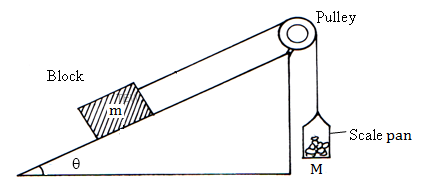
\includegraphics[width=10cm]{./img/coefficient-friction-1.png}
\caption{Coefficient of Friction practical setup}
\label{fig:coefficient-friction-1}
\end{figure}

\section{Analysis and Interpretation}
\begin{enumerate}
\item For each value of $\theta$ calculate the coefficient of friction of the wooden block using the equation:

\begin{center}
$\text{coefficient of friction }(\mu)=\cfrac{Mg-mg\sin \theta}{mg\cos \theta}$
\end{center}
 
\item Comment about the values of $\mu$.
\end{enumerate}

\section{Conclusion}
From the experiment, what is the coefficient of friction between the wooden block and the inclined plane?

\section{Questions for Discussion}
\begin{enumerate}
\item If the inclined plane were rougher, would you obtain the same value of $\mu$?
\item If the angle of inclination remains constant, but the weight of the block on the inclined plane increases, what would have to happen to the weight on the scale pan to obtain a proper value for the coefficient of friction?
\item What is the purpose of increasing the angle of inclination in this experiment?
\end{enumerate}

\section{Reflection and Self Assessment}
\begin{enumerate}
\item Were there any problems encountered during the experiment? If yes, explain.
\item How could you use the knowledge of this experiment to simplify the job of moving a large pile of bricks across a floor?
\item Why is it difficult to walk on a slippery floor?
\end{enumerate}